\section{Background and Previous Work}
\label{sec:locvqallm_background}

% introductory paragraph
\gls{vqa} is centered on developing models capable of answering questions about specific images~\cite{antol2015vqa}. This task is particularly challenging within the medical domain due to factors such as a scarcity of annotated data~\cite{Nguyen19,liu2019effective}, the wide variety of imaging modalities and anatomical regions~\cite{gupta2021hierarchical}, as well as the unique characteristics of medical images and terminology, all of which necessitate specialized expertise~\cite{liu2019effective,zhan2020medical}. Furthermore, approaches that leverage the detection of natural objects, which have significantly improved performance in the analysis of natural images~\cite{anderson2018bottom}, are less straightforward when applied to medical imagery~\cite{gupta2021hierarchical}.

Historically, models for \gls{medvqa} treated visual and textual information independently, later merging these features through various fusion techniques. This composite data would then be input into a classifier to determine the most probable answer. However, recent developments in transformer-based models~\cite{vaswani2017attention}, including advancements in~\glspl{llm}, have led to a notable shift in \gls{vqa} strategies. These advancements have paved the way for the adoption of \glspl{mllm} that integrate both visual and textual data more seamlessly, a trend that is emerging in both general~\cite{yin2023survey,tong2024eyes,zhang2024mm} and medical \gls{vqa}~\cite{seenivasan2023surgicalgpt,zhang2023pmc} applications.

% About models not actually understanding images
Despite the remarkable adoption of \glspl{mllm}, recent research has raised concerns about the quality of their visual capabilities (Fig.~\ref{fig:locvqallm_examples_gpt_4v}). This issue primarily arises from the pre-training process of the visual component, which typically relies on models like CLIP~\cite{radford2021learning}. Surprisingly, \glspl{mllm} can perceive certain visually distinct images as similar, a phenomenon that human observers readily recognize as different~\cite{tong2024eyes}. These visual understanding failures were also observed in \gls{vqa} models before the widespread adoption of \glspl{mllm}~\cite{goyal2017making,hudson2019gqa,ribeiro2019red,selvaraju2020squinting}.
\begin{figure}[!h]
\begin{center}
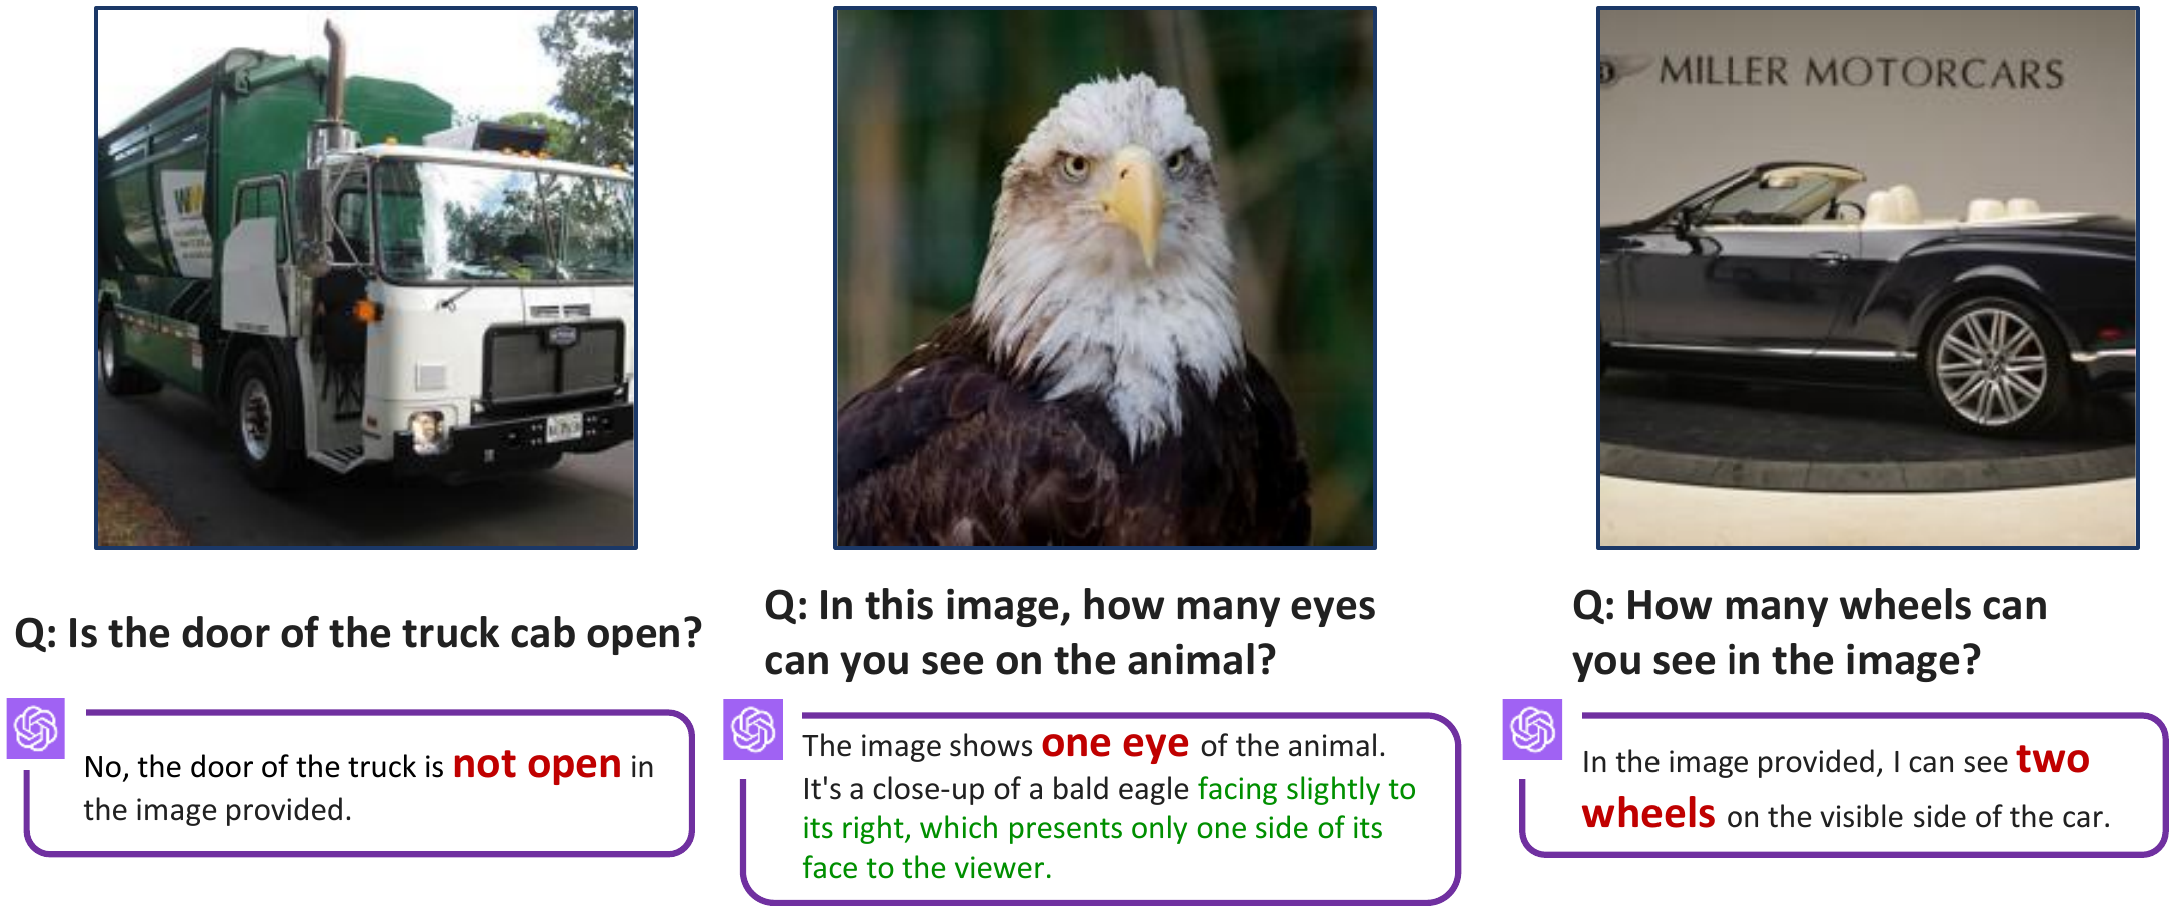
\includegraphics[width=0.9\textwidth]{Figures/Part1_LocVQA/02_llm/examples_gpt_4v.png}
\caption{Examples of visual understanding failures using GPT-4V for the VQA task. From~\cite{tong2024eyes}.}
\label{fig:locvqallm_examples_gpt_4v}
\end{center}
\end{figure}

To enhance explainability in the visual component of \gls{medvqa}, the work in~\cite{tascon2023localized} proposes a novel approach using the formulation of \textit{localized questions}~\cite{tascon2023localized}. These questions allow fine-grained probing of images by focusing on user-defined regions rather than the entire image and facilitate a \textit{compositional evaluation} of the model's reasoning abilities.
To enable such localized questions, the region to query is encoded and directly integrated into the attention mechanism of the model. By doing so, the model gains access to context relevant to answering the question. Alternatively, other proposed strategies include providing the model with a restricted region of the image~\cite{tascon2022consistency} or relying on the language component of the \gls{vqa} model to interpret region coordinates directly included in the question~\cite{vu2020question}. Notably,~\cite{mani2020point} limits spatial focus by considering only certain bounding boxes produced by an object detector. Yet all of these methods suffer from the same common limitation: \glspl{mllm} cannot directly be integrated into these schemes to leverage their benefits for Med-VQA.

%For example, consider the car image on the right in Fig.~\ref{fig:examples_gpt_4v}. Instead of asking a generic question like "How many wheels can you see?" about the entire image, we can pose the same question specifically for regions that do not contain any wheels. 


To this end, we propose to overcome this challenge by introducing a novel approach, namely {\it Targeted Visual Prompting}. By carefully designing a prompt that provides both global and local visual tokens relative to the region of interest defined by the user, our method allows the full advantage of the \gls{mllm} to enhance the performance of the \gls{vqa} model. To validate the effectiveness of our method, we conduct exhaustive experiments across multiple datasets. Our results demonstrate clear performance benefits compared to previously proposed methods, all achieved without introducing additional parameters to the model. %By bridging the gap between MLLMs and domain-specific requirements, Targeted Visual Prompting represents a significant step forward in Med-VQA research.


%In this paper, we aim at advancing visual reasoning in the context of Med-VQA. Our method addresses the limitations of existing MLLMs by enabling fine-grained analysis. 

%The existing approaches, such as context-blind models~\cite{tascon2022consistency}, specific multi-glimpse guided-attention mechanisms~\cite{tascon2023localized,vu2020question}, and object detection requirements~\cite{mani2020point}, exhibit a common limitation: they are not directly applicable to MLLMs. To overcome this challenge, we propose **Targeted Visual Prompting**. In this innovative approach, a carefully designed prompt provides both global and local visual tokens relative to the region of interest defined by the user.